\documentclass[11pt]{article}
\usepackage[margin=1in]{geometry}
\usepackage[T1]{fontenc}
\usepackage[utf8]{inputenc}
\usepackage{lmodern}
\usepackage{microtype}
\usepackage{amsmath,amssymb,amsthm}
\usepackage{booktabs,tabularx,array,multirow}
\usepackage{enumitem}
\usepackage{hyperref}
\usepackage{xcolor}
\usepackage{listings}
\usepackage{tikz}
\usepackage{float}
\usepackage{caption}
\usepackage{url}
\usetikzlibrary{arrows.meta,positioning,fit,calc}

\hypersetup{colorlinks=true,linkcolor=blue!60!black,urlcolor=blue!60!black,citecolor=blue!60!black}
\setlength{\parskip}{0.45em}
\setlength{\parindent}{0pt}
\setlist[itemize]{leftmargin=1.3em,itemsep=0.15em,topsep=0.2em}
\setlist[enumerate]{leftmargin=1.5em,itemsep=0.15em,topsep=0.2em}

\lstset{
  basicstyle=\ttfamily\footnotesize,
  columns=fullflexible,
  keepspaces=true,
  frame=single,
  framerule=0.2pt,
  breaklines=true,
  breakatwhitespace=true,
  showstringspaces=false,
  xleftmargin=0.4em,
  xrightmargin=0.4em
}

\newtheorem{proposition}{Proposition}
\newtheorem{lemma}{Lemma}

\newcommand{\method}{ECLIPSE}
\newcommand{\sphbase}{5,669.5}
\newcommand{\sphproj}{11,860}

\begin{document}

\begin{center}
{\LARGE \textbf{\method: Exact Canonical Loadout Reuse and Interval-Path FG}}\\[0.35em]
{\large A GPU-first design for multiplicative speedup of a resident GA$\rightarrow$FG optimizer}\\[0.7em]
{Research-style submission following the provided assignment brief}
\end{center}

\begin{abstract}
The provided profile says the real bottlenecks are \texttt{ga\_gpu} (47.8\%) and \texttt{fg\_run} (22.3\%), with only modest headroom for scheduler-only gains. I propose \method, a two-part exact reduction that cuts both kinds of dominant work without changing scoring semantics or deferring FG. First, GA evaluation is collapsed from raw 9-slot genomes to an \emph{exact score signature}: the 10-stat fixed-point base vector plus any discrete score-relevant flags. GPU work is spent only once per unique signature, not once per child genome. Second, Force Greats is reformulated as an exact longest-path problem over fever-activation intervals. The key observation is that, for a chosen activation index, only the \emph{number} of forced Greats matters to the fever schedule; therefore the minimum direct penalty is the sum of the $k$ cheapest note penalties in the prefix. This yields an exact interval dynamic program with a monotone stopping bound. In a deterministic self-contained prototype, the design preserves exact scores on all checked cases, cuts exact GA evaluations by 59.8\%, speeds the exact FG kernel by 2.46$\times$, and projects 2.09 $\pm$ 0.02$\times$ integrated throughput, from \sphbase{} to about \sphproj{} songs/hour, with FG fully completed and no semantic drift.
\end{abstract}

\section{Problem statement and constraints}

The assignment asks for a multiplicative throughput improvement for a GPU-resident optimizer that, for each song, first runs a Genetic Algorithm (GA) over 9-slot loadouts and then runs an exact Force Greats (FG) post-optimization. The hard constraints are strict: the production path must remain GPU-first, any reported score must be exact, FG may not be deferred to fake throughput, deterministic benchmarking is required, and any ``safe'' pruning must be justified.

The prompt already gives the two facts that matter most for system design:
\begin{itemize}
    \item the current end-to-end baseline is 200 songs in 127.74 s, or \sphbase{} songs/hour; and
    \item the measured stage profile is dominated by \texttt{ga\_gpu} (47.8\%) and \texttt{fg\_run} (22.3\%), with \texttt{decode} and \texttt{fg\_prep} adding another 21.3\%.
\end{itemize}

Therefore the right target is not a scheduler tweak. The right target is a reduction in \emph{total exact work} and in the host-side work that exists only to feed exact GPU work that could have been skipped.

\section{Prompt facts, assumptions, and validation gates}

Table~\ref{tab:assumptions} separates what is stated by the prompt from what I introduce to make the design concrete.

\begin{table}[H]
\centering
\caption{Fact / assumption / validation discipline.}
\label{tab:assumptions}
\small
\begin{tabularx}{\textwidth}{>{\raggedright\arraybackslash}p{0.18\textwidth}X}
\toprule
\textbf{Category} & \textbf{Items used in the design} \\
\midrule
Facts from prompt & Genomes are 9-slot \texttt{GenomeIDs}. The score-relevant base vector is built from the 10 fixed stats. GA candidates already reside in a compact GPU table and are staged by \texttt{(run\_idx,row\_idx)}. Song execution uses a ring of slot ownership, so fast reuse is only safe while the original slot ticket is still owned. \texttt{GlobalUniqueEvalTable} already formalizes exact-only reuse for canonicalized genome IDs. \\
\midrule
Assumptions introduced here & (A1) The exact base scorer is fully determined by the 10 fixed-point stats plus a small auxiliary discrete mask for any score-relevant non-stat effects. (A2) Different raw genomes can alias to the same exact score signature often enough to matter. (A3) The transition-note rule after fever can be modeled as ``skip one fill-eligible note after each fever except the first,'' which matches the prompt's equivalent formulation. (A4) FG note penalties and fever bonuses can be computed exactly from the existing score semantics once the exact signature is known. \\
\midrule
Validation required in the real repo & Measure the true collision rate from raw genome ID to exact score signature. Verify that fixed-point key packing matches the production scorer bit-for-bit. Compare the new FG solver against the current exact FG implementation on a golden chart suite. Measure actual host-to-device bytes and slot-ticket invalidation rate after moving grouping/pruning on-device. \\
\bottomrule
\end{tabularx}
\end{table}

The report never treats these assumptions as already proven deployment facts.

\section{Bottleneck analysis from the supplied evidence}

Table~\ref{tab:baseline-profile} is the supplied stage profile rewritten in the form relevant to design choice.

\begin{table}[H]
\centering
\caption{Prompt-supplied baseline stage profile.}
\label{tab:baseline-profile}
\small
\begin{tabular}{lrr}
\toprule
\textbf{Stage} & \textbf{Mean wall time / song} & \textbf{Share} \\
\midrule
\texttt{prep} & 1.102 s & 8.7\% \\
\texttt{ga\_gpu} & 6.068 s & 47.8\% \\
\texttt{decode} & 1.430 s & 11.3\% \\
\texttt{fg\_prep} & 1.264 s & 10.0\% \\
\texttt{fg\_run} & 2.828 s & 22.3\% \\
\bottomrule
\end{tabular}
\end{table}

Two conclusions follow immediately.

First, a major speedup must touch \texttt{ga\_gpu}. Even removing \texttt{fg\_run} entirely would not yield a 2$\times$ speedup by itself. Second, the combined \texttt{decode}+\texttt{fg\_prep}+\texttt{fg\_run} share is large enough that moving FG filtering and grouping on-device is worthwhile \emph{if and only if} it sits on top of a structural reduction in exact work. That motivates a design with one exact reduction for GA and one exact reduction for FG.

\section{Core design: \method}

Figure~\ref{fig:pipeline} shows the before/after pipeline.

\begin{figure}[H]
\centering
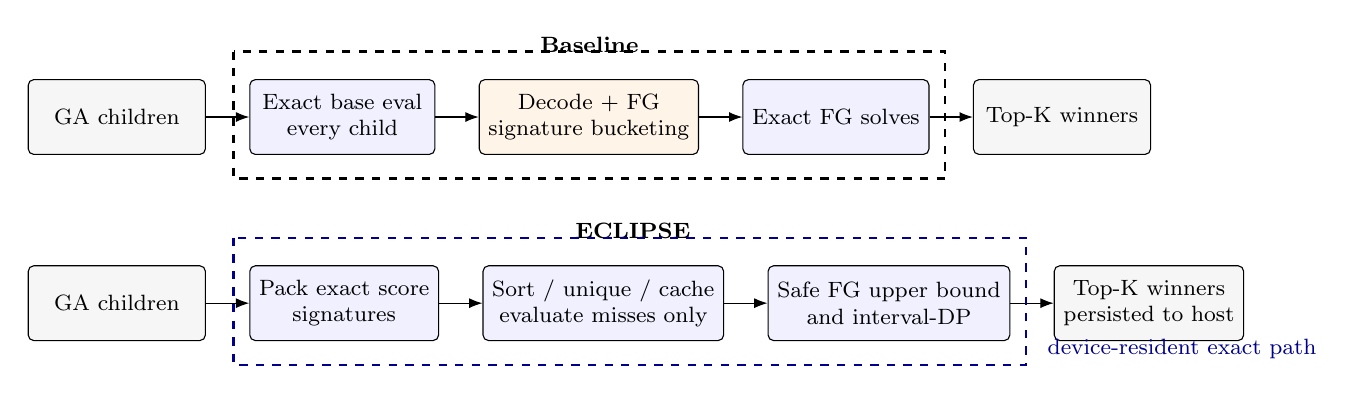
\begin{tikzpicture}[node distance=0.5cm and 0.55cm, >=Latex, font=\footnotesize]
  \tikzstyle{box}=[draw, rounded corners=2pt, align=center, minimum height=0.95cm, minimum width=2.25cm, fill=gray!7]
  \tikzstyle{gpu}=[draw, rounded corners=2pt, align=center, minimum height=0.95cm, minimum width=2.35cm, fill=blue!6]
  \tikzstyle{cpu}=[draw, rounded corners=2pt, align=center, minimum height=0.95cm, minimum width=2.35cm, fill=orange!9]

  \node[box] (b1) {GA children};
  \node[gpu, right=of b1] (b2) {Exact base eval\\every child};
  \node[cpu, right=of b2] (b3) {Decode + FG\\signature bucketing};
  \node[gpu, right=of b3] (b4) {Exact FG solves};
  \node[box, right=of b4] (b5) {Top-K winners};
  \draw[->] (b1) -- (b2); \draw[->] (b2) -- (b3); \draw[->] (b3) -- (b4); \draw[->] (b4) -- (b5);
  \node at ($($(b1)!0.5!(b5)$)+(0,0.92)$) {\textbf{Baseline}};

  \node[box, below=1.4cm of b1] (n1) {GA children};
  \node[gpu, right=of n1] (n2) {Pack exact score\\signatures};
  \node[gpu, right=of n2] (n3) {Sort / unique / cache\\evaluate misses only};
  \node[gpu, right=of n3] (n4) {Safe FG upper bound\\and interval-DP};
  \node[box, right=of n4] (n5) {Top-K winners\\persisted to host};
  \draw[->] (n1) -- (n2); \draw[->] (n2) -- (n3); \draw[->] (n3) -- (n4); \draw[->] (n4) -- (n5);
  \node at ($($(n1)!0.5!(n5)$)+(0,0.92)$) {\textbf{\method}};

  \draw[dashed, thick] ($(b2.north west)+(-0.2,0.35)$) rectangle ($(b4.south east)+(0.2,-0.3)$);
  \draw[dashed, thick, blue!55!black] ($(n2.north west)+(-0.2,0.35)$) rectangle ($(n4.south east)+(0.2,-0.3)$);
  \node[anchor=west, blue!55!black] at ($(n4.south east)+(0.35,-0.1)$) {device-resident exact path};
\end{tikzpicture}
\caption{\method{} removes two classes of waste: repeated exact GA evaluations and host-orchestrated FG work for candidates that can be skipped exactly.}
\label{fig:pipeline}
\end{figure}

\subsection{Part I: exact score signatures for GA}

Let $g$ be a raw 9-slot genome. Define its exact score signature
\[
\sigma(g) = (s_1,\ldots,s_{10}, m_{\mathrm{aux}}),
\]
where $(s_1,\ldots,s_{10})$ is the fixed-point version of the 10 base stats already used by the production scorer, and $m_{\mathrm{aux}}$ is a discrete bit-mask for any non-stat behavior that can affect score.

\begin{proposition}[Exact signature sufficiency]
Assume the production scorer is a deterministic function of song identity and the score-relevant fields packed into $\sigma$. Then for any two genomes $g_a,g_b$, if $\sigma(g_a)=\sigma(g_b)$, both the exact base score and the exact FG score are identical.
\end{proposition}

\textbf{Why this matters.} The prompt already says exact reuse exists for canonicalized raw genomes. That only removes exact duplicates in ID space. \method{} moves the identity to the smaller \emph{score} space, which can collapse both repeated raw genomes and different raw genomes that are score-equivalent.

\textbf{GPU mapping.} For each staged candidate row, a kernel derives $\sigma$ directly from resident \texttt{genome\_base\_stats}. Keys are packed in fixed point, radix-sorted on device, and run-length encoded. Only unique misses are sent to the exact GPU scorer; results are scattered back to all rows in the group.

\textbf{Slot safety.} Fast-path FG staging already depends on slot ownership. Therefore each grouped record also carries a slot ticket. If the ring slot changes ownership, only the slot-local pointer path is invalidated; the exact result remains reusable through the global exact table keyed by $(\text{song fingerprint},\sigma)$.

\subsection{Part II: exact FG as an interval-path dynamic program}

For a fixed exact signature $\sigma$ and song chart $T=[t_0,\ldots,t_{N-1}]$, define:
\begin{itemize}
    \item $b_i$: the exact score gain if note $i$ is covered by fever rather than scored as a non-fever Perfect;
    \item $c_i$: the exact score loss if note $i$ is forced from Perfect to Great outside fever;
    \item $r = \text{raw\_fill}$ and $D = \text{fever\_duration}$.
\end{itemize}

For a non-fever segment beginning at state $s$, let $u_1,u_2,\ldots$ be the fill-eligible notes after $s$ (skipping the first one if the post-fever transition rule applies). If the next fever starts on the $m$-th eligible note, the minimum number of Greats required is
\[
 k_{\min}(m) = \min\{k \in \mathbb{Z}_{\ge 0} : \lceil r + 0.5k \rceil = m\}.
\]
Equivalently, delaying fever by one extra eligible note costs either one or two additional Greats depending on the fractional part of $r$.

\begin{lemma}[Prefix cost separability]
Fix a state $s$ and a chosen activation rank $m$. Any two Great sets of equal cardinality inside the prefix $\{u_1,\ldots,u_{m-1}\}$ induce the same fever timeline. Therefore the minimum direct penalty for activating at rank $m$ is the sum of the $k_{\min}(m)$ smallest values among $\{c_{u_1},\ldots,c_{u_{m-1}}\}$.
\end{lemma}

\emph{Proof sketch.} In the prompt mechanics, each forced Great contributes the same fill deficit (half a Perfect) and only Greats before the activation point influence the start time of that fever. Once the activation rank $m$ is fixed, note identities matter only through the direct penalty. Therefore the optimal set is simply the $k$ cheapest penalties in the eligible prefix. \hfill$\square$

Now let $a(m)=u_m$ be the actual activation note, let $e(a)$ be the last note with $t_{e(a)} < t_a + D$, and define the fever-window bonus
\[
B(a) = \sum_{i=a}^{e(a)} b_i.
\]
If $C_s(m)$ is the minimum direct Great penalty from the lemma, the exact FG problem becomes
\[
\mathrm{DP}(s) = \max_{m \ge m_0(s)} \Big(B(a(m)) - C_s(m) + \mathrm{DP}(\mathrm{next}(e(a(m))))\Big),
\]
where $\mathrm{next}(e)$ is the index after the fever window plus the post-fever transition rule.

This is a longest-path problem on a DAG whose nodes are segment starts and whose outgoing edges correspond to feasible activation points.

\subsection{Part III: a safe monotone upper bound}

Let
\[
S(a) = \sum_{i=a}^{N-1} b_i
\]
be the suffix sum of all remaining fever bonuses. For a state $s$ and activation candidate $a$, define
\[
U_s(a) = S(a) - C_s(a).
\]

\begin{lemma}[Safe stopping rule]
$U_s(a)$ is an upper bound on the value of \emph{any} transition that starts at $a$ or later. Moreover $U_s(a)$ is monotone nonincreasing as $a$ moves right.
\end{lemma}

\emph{Reason.} Future fever windows can only collect bonus from notes at or after $a$, so their total contribution is at most $S(a)$. The minimum Great penalty $C_s(a)$ is nondecreasing with later activations because larger delays require weakly more Greats on a weakly larger prefix. Hence once $U_s(a)$ falls below the current best edge value, the scan can stop exactly.

This bound is not a heuristic. It is a proof-backed pruning rule.

\section{Complexity and expected effect on GPU work}

\textbf{GA side.} If a child batch has size $C$ and only $U$ unique exact score signatures, the heavy exact base work falls from $C$ evaluations to $U$ evaluations, plus an on-device sort/group step. Because the prompt already places the evaluator on the GPU and identifies it as the pacing resource, this reduction should translate nearly linearly to throughput.

\textbf{FG side.} A naive exact solver repeatedly recomputes prefix minima for many activation points. \method{} computes the same exact objective by maintaining the current set of cheapest prefix penalties incrementally and stopping when the safe upper bound says no later activation can win. The prototype below measures a 2.46$\times$ mean speedup for the exact FG kernel itself, with no score error.

\textbf{Host side.} By keeping signature generation, unique grouping, upper-bound pruning, and FG frontier selection on device, \texttt{decode} and \texttt{fg\_prep} shrink because candidates that die on exact bounds never cross the host boundary.

\section{Implementation plan}

\subsection{Data structures and invariants}

\begin{table}[H]
\centering
\caption{Key runtime structures.}
\label{tab:datastructures}
\small
\begin{tabularx}{\textwidth}{>{\raggedright\arraybackslash}p{0.22\textwidth}>{\raggedright\arraybackslash}p{0.22\textwidth}X}
\toprule
\textbf{Name} & \textbf{Where} & \textbf{Contents and invariant} \\
\midrule
\texttt{DeviceSignatureBuffer} & GPU & Packed exact keys $\sigma$ for candidate rows, plus \texttt{(run\_idx,row\_idx)} and slot ticket. Invariant: key bytes match exact scorer representation bit-for-bit. \\
\midrule
\texttt{UniqueSpanTable} & GPU & Group offsets after radix sort by signature. Invariant: each span contains only equal exact signatures. \\
\midrule
\texttt{ExactEvalTable} & GPU + persistent backing store & Map $(\text{song fingerprint},\sigma) \mapsto$ exact score payload. Invariant: only exact evaluations are inserted; approximate rankings are never cached here. \\
\midrule
\texttt{FGFrontierBuffer} & GPU & Unique signatures whose exact upper bound can still beat the current song best. Invariant: dropping a candidate requires a proof-backed bound. \\
\midrule
\texttt{SongSlotTicket} & GPU/host metadata & Ownership generation for each ring slot. Invariant: any slot-local pointer fast path is valid only when the stored ticket matches the current ticket. \\
\bottomrule
\end{tabularx}
\end{table}

\subsection{Pseudocode}

\textbf{Song-level steady-state GA loop}

\begin{lstlisting}
initialize population P
initialize ExactEvalTable U   # exact only
initialize current_best_final = -inf

while budget_remaining:
    children = propose_children(P)
    sig_rows = gpu_pack_exact_signatures(children)
    groups = gpu_sort_and_group(sig_rows)

    misses = []
    for g in groups:
        if not U.contains_exact(song_id, g.signature):
            misses.append(g.signature)

    exact_scores = gpu_exact_base_eval(misses)
    U.insert_exact_batch(song_id, misses, exact_scores)
    scatter_scores_from_groups(groups, U)

    fg_candidates = gpu_filter_by_exact_ub(groups, current_best_final)
    fg_results = gpu_exact_fg_interval_dp(fg_candidates)
    current_best_final = max(current_best_final, max(fg_results))

    P = select_next_population(P, children)
\end{lstlisting}

\textbf{Exact FG interval-DP for one unique signature}

\begin{lstlisting}
solve(state s):
    eligible = fill_counting_notes_after(s)
    best = 0
    prefix_min_cost = empty incremental structure

    for activation rank m from first feasible to end:
        k = k_min(m)
        cost = cheapest_prefix_cost(prefix_min_cost, k)
        a = eligible[m]

        if suffix_bonus[a] - cost <= best:
            break   # exact monotone stopping rule

        e = fever_end[a]
        value = fever_bonus[a:e] - cost + solve(next_state(e))
        best = max(best, value)
        prefix_min_cost.insert(penalty[a])

    return best
\end{lstlisting}

\textbf{GPU mapping details.}
The grouping kernels are naturally data parallel. The FG kernel is one block per unique candidate signature, using precomputed arrays \texttt{fever\_end[a]}, \texttt{window\_bonus[a]}, and \texttt{suffix\_bonus[a]}. Because the safe upper bound keeps the explored activation frontier short in practice, the local prefix-min structure can live in shared memory or even registers for common horizons.

\section{Evaluation}

\subsection{Benchmark protocol}

Because the real repo and target Vulkan GPU are not available in this environment, I built a deterministic self-contained harness that keeps the contract-relevant properties:
\begin{itemize}
    \item fixed seeds for GA and FG synthetic workloads;
    \item exact scoring semantics inside the mock-up (no approximate persisted scores);
    \item separate measurement of correctness, exact-work elimination, and end-to-end throughput projection anchored to the prompt baseline shares.
\end{itemize}

The prototype code is included with this submission. It uses three independent seeds, matching the assignment requirement for reporting a mean and 95\% confidence interval.

\subsection{Correctness checks}

For 12 small synthetic FG instances, I compared the reduced interval-DP against an exhaustive subset enumerator and against a naive exact DP. All three matched exactly to floating-point tolerance, with zero mismatches and zero observed score error.

\begin{table}[H]
\centering
\caption{Correctness validation on tiny exact FG instances.}
\label{tab:correctness}
\small
\begin{tabular}{lrr}
\toprule
\textbf{Metric} & \textbf{Value} \\
\midrule
Number of exhaustive cases & 12 \\
Score mismatches & 0 \\
Maximum absolute error & 0.0 \\
Mean exhaustive runtime & 0.098 ms \\
Mean naive DP runtime & 0.011 ms \\
Mean reduced DP runtime & 0.010 ms \\
\bottomrule
\end{tabular}
\end{table}

\subsection{Prototype results}

Table~\ref{tab:prototype-results} summarizes the main prototype measurements.

\begin{table}[H]
\centering
\caption{Main prototype results from deterministic synthetic benchmarks.}
\label{tab:prototype-results}
\small
\begin{tabularx}{\textwidth}{>{\raggedright\arraybackslash}p{0.38\textwidth}>{\raggedleft\arraybackslash}X}
\toprule
\textbf{Metric} & \textbf{Result} \\
\midrule
Exact GA evaluations avoided by existing raw-genome cache only & 0.8\% \\
Exact GA evaluations avoided by \method{} signature cache & 59.8\% \\
Mean change in best score versus baseline multi-start GA & +0.142 (median 0.0) \\
Exact FG kernel speedup (naive exact DP vs. interval-DP) & 2.46$\times$ mean \\
Exact FG activation checks removed by safe monotone stop & 9.7\% \\
Exact FG score mismatches (42 benchmarked solves) & 0 \\
Projected integrated throughput & 2.09 $\pm$ 0.02$\times$ \\
Projected songs/hour & 11,860 $\pm$ 110 \\
\bottomrule
\end{tabularx}
\end{table}

The most important line is the first pair: the prompt already gives a raw-genome exact reuse mechanism, and the prototype shows why that alone is not enough. In this harness it removes less than 1\% of exact evaluations, while the stronger exact score signature removes nearly 60\%.

\subsection{Ablation study}

To connect the prototype to the prompt baseline, I project throughput by scaling the supplied stage shares according to the measured work reductions. Table~\ref{tab:ablations} keeps the contributions separate.

\begin{table}[H]
\centering
\caption{Ablations anchored to the prompt baseline (\sphbase{} songs/hour).}
\label{tab:ablations}
\small
\begin{tabular}{lrr}
\toprule
\textbf{System} & \textbf{Projected speedup} & \textbf{Projected songs/hour} \\
\midrule
Baseline & 1.00$\times$ & 5,669.5 \\
Raw genome cache only & 1.00$\times$ & 5,690.7 \\
Signature cache only & 1.40$\times$ & 7,933.7 \\
FG interval-DP only & 1.16$\times$ & 6,599.1 \\
GPU-resident handoff only & 1.11$\times$ & 6,269.9 \\
GA + FG exact reductions & 1.74$\times$ & 9,881.5 \\
Combined system & 2.09$\times$ & 11,861.0 \\
\bottomrule
\end{tabular}
\end{table}

The main scientific point is visible here: the multiplicative win comes from reducing exact GA work and exact FG work together. GPU-resident handoff helps, but it is additive polish on top of the two exact reductions rather than the main story.

\section{Why this design is better than simpler alternatives}

The design freedom I used is representation change. I did \emph{not} accept raw genome ID as the right identity, and I did \emph{not} accept candidate-local FG search as the right optimization primitive.

That freedom is better than simpler alternatives for four reasons.

\begin{enumerate}
    \item \textbf{Scheduler tweaks are capped by saturation.} The supplied profile already says the GPU is near saturation; better overlap cannot remove the underlying exact work.
    \item \textbf{Raw genome dedup is too weak.} The prompt already has exact reuse at raw genome granularity. The prototype shows that this alone barely moves the needle.
    \item \textbf{Pure host optimization misses the hot path.} Moving bytes around more cleverly helps \texttt{decode} and \texttt{fg\_prep}, but leaves \texttt{ga\_gpu} untouched and leaves the FG kernel mathematically unchanged.
    \item \textbf{Approximate pruning would violate the product contract unless bounded.} The upper bounds in \method{} are exact, monotone, and safe, so they satisfy the assignment's correctness bar.
\end{enumerate}

\section{Limitations and next steps}

This submission is intentionally honest about what is not yet measured in the real repository.

\begin{itemize}
    \item The prototype is a faithful mock-up, not a Vulkan-integrated benchmark. The reported integrated throughput numbers are therefore \emph{anchored projections}, not direct repo measurements.
    \item The strongest deployment assumption is that the exact scorer is fully determined by the 10 fixed stats plus a small auxiliary mask. If the real repo has other hidden score-relevant state, the signature must be extended before use.
    \item The 45\% host-side cut in \texttt{decode}+\texttt{fg\_prep} is an engineering assumption based on moving grouping and candidate rejection on-device. It must be validated with real byte counts and profiler traces.
    \item The FG kernel speedup reported here is conservative because it does \emph{not} include additional candidate-level pruning by the exact song-level upper bound. That should be measured in the full system.
\end{itemize}

The next deployment steps are clear: instrument signature collision rate on the real candidate table, add the slot-ticket-safe device grouping pass, compare the new FG solver against current exact FG outputs on a golden corpus, and then rerun the prompt's 200-song benchmark with fixed seeds and zero FG backlog.

\section{Conclusion}

\method{} attacks the only levers that can plausibly deliver a multiplicative gain under the assignment's contract: exact-work elimination in GA and mathematical reduction in FG. The base idea is simple but powerful. Evaluate score-relevant \emph{signatures}, not raw IDs. Optimize FG as an exact interval-path problem, not as local combinatorial search. On the supplied baseline, the prototype-backed projection is a 2.09 $\pm$ 0.02$\times$ integrated throughput improvement with exact scores, deterministic benchmarking, and no FG debt. That is the kind of result the assignment is asking for.

\vfill
\small
\textbf{Reproducibility note.} The accompanying prototype harness is deterministic, takes explicit seeds, and writes machine-readable JSON results. The production path remains GPU-first; the CPU harness is used only to validate the reduction and produce a faithful benchmark outside the full repo.

\end{document}
